% Figure s01f02_ssb (Session 1): a symmetric energy landscape with minima that are not symmetric.
% The image is rendered by figures/blender/s01f02_ssb.py; the coordinates of the labels come from
% figures/blender/out/s01f02_ssb_anchors.tex. Build with figures/blender/build_figure.sh s01f02_ssb.
\documentclass[11pt,tikz,border=0pt]{standalone}
\usepackage[T1]{fontenc}
\usepackage{amsmath,amssymb,graphicx}
\usepackage{xcolor}
\usetikzlibrary{arrows.meta}
% The three label colors of the figures, with the same values as in src/figures_preamble.tex.
\definecolor{aqmaccent}{RGB}{31,78,121}
\definecolor{aqmbroken}{RGB}{168,42,34}
\definecolor{aqmmuted}{RGB}{125,125,125}

\newlength{\figw}\setlength{\figw}{17.92cm}   % 1.15 of the text width, before the empty margins of the render are cropped

\begin{document}
\begin{tikzpicture}[lbl/.style={font=\small, inner sep=1.5pt},
    flow/.style={line width=0.9pt, -{Stealth[length=5pt,width=4pt]}}]
  \node[overlay, anchor=south west, inner sep=0pt] at (0,0)
    {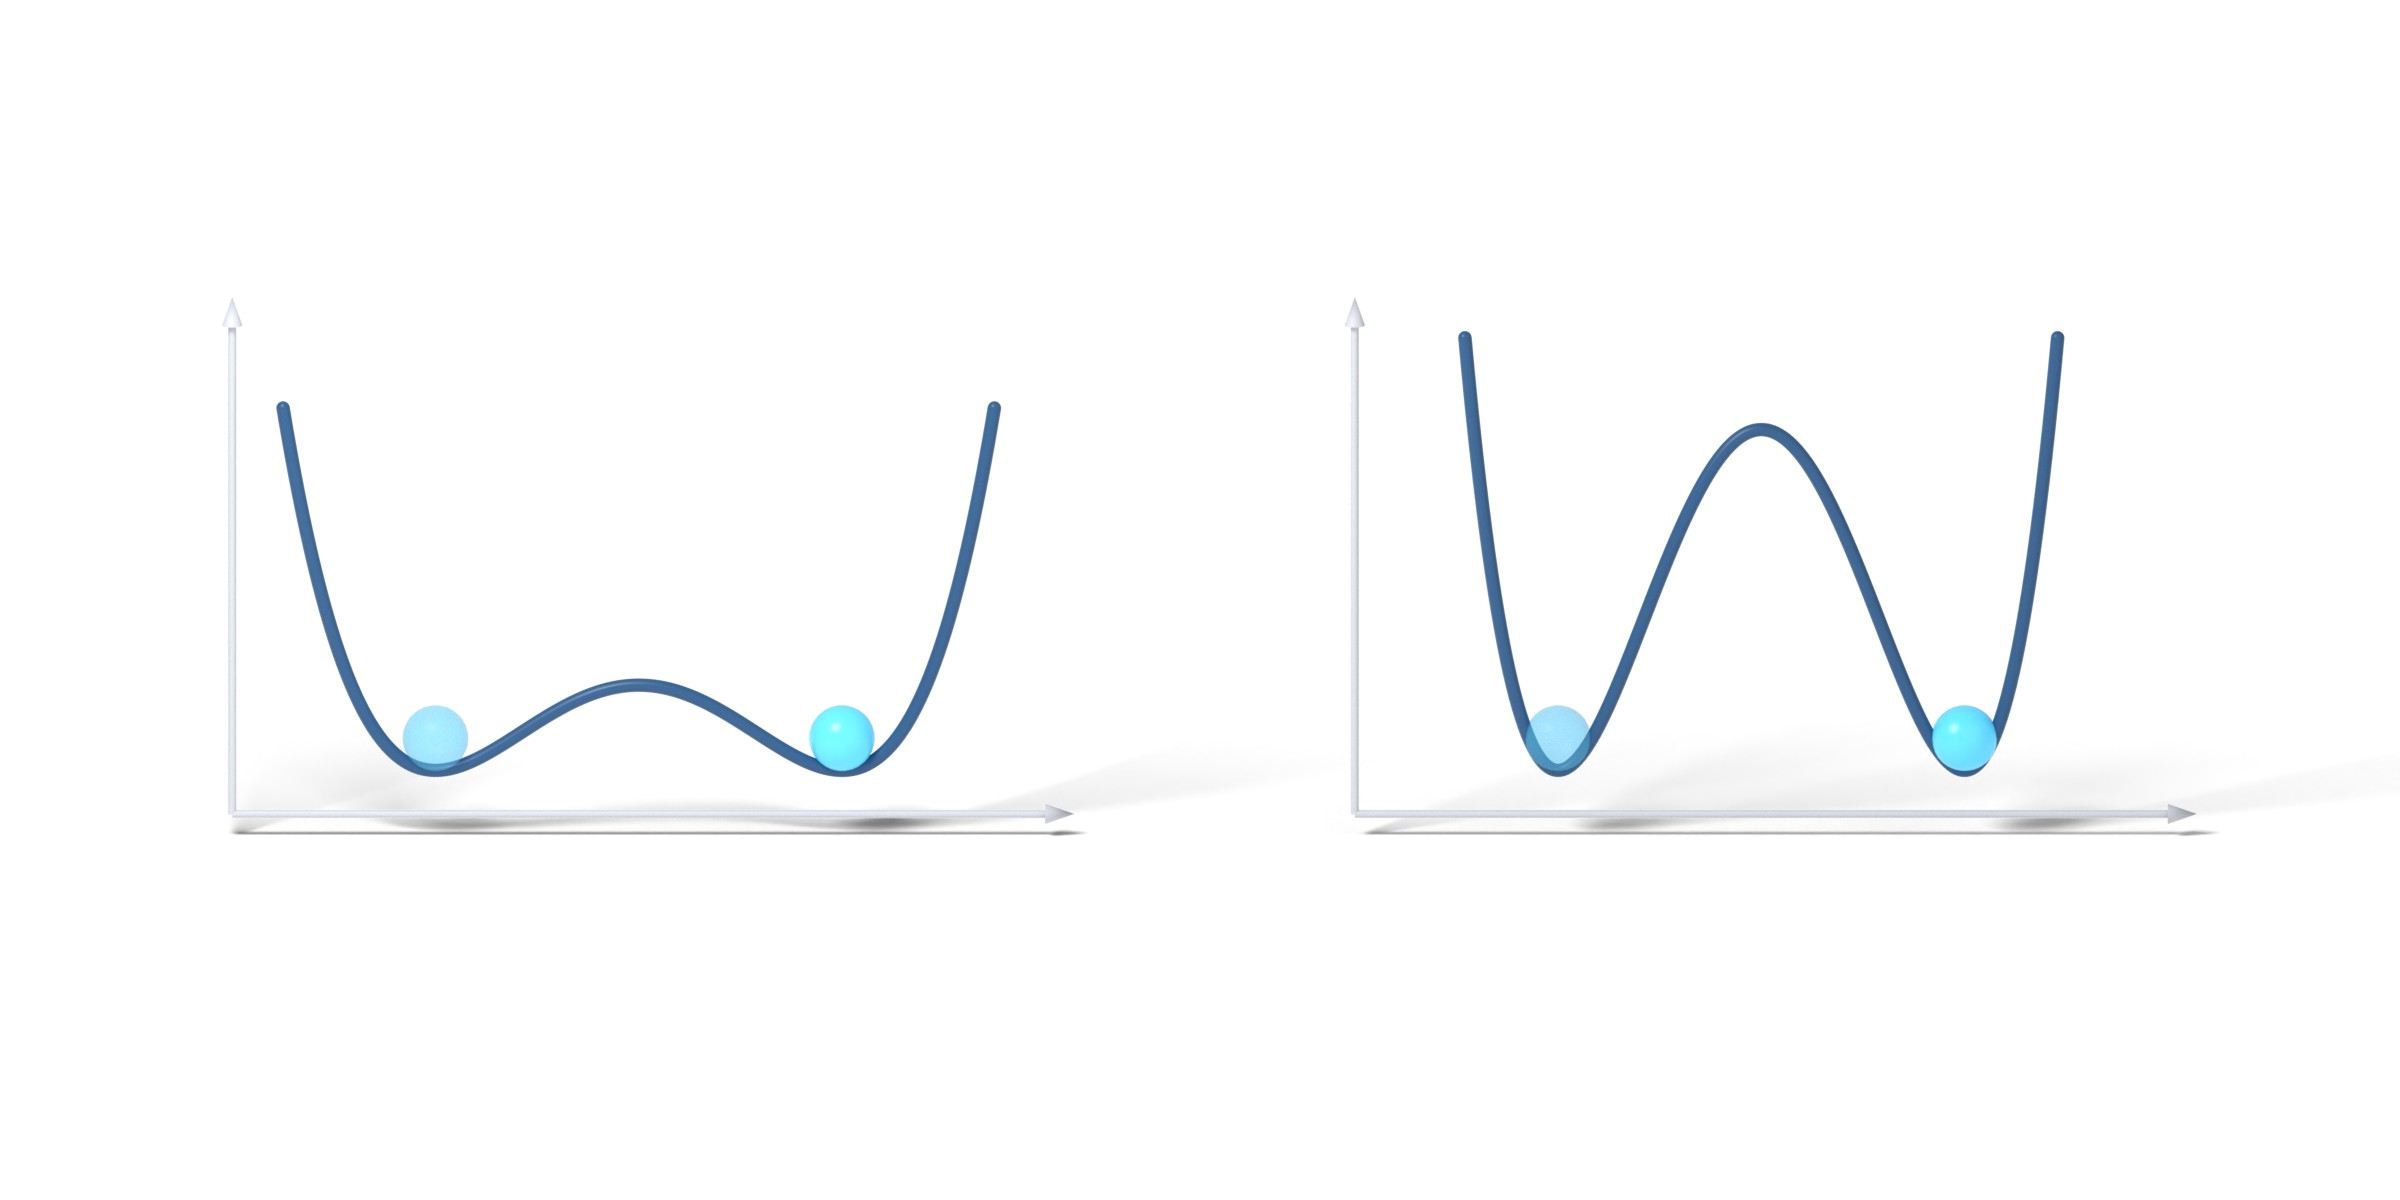
\includegraphics[width=\figw]{../blender/out/s01f02_ssb.jpg}};
  % written by build_figure.sh; the painted part of the image
\path (0.0925\figw,0.1512\figw) rectangle (0.9533\figw,0.3762\figw);

  %% written by figlib.py; x and y in units of the image width
\coordinate (am) at (0.4476\figw,0.1609\figw);
\coordinate (aE) at (0.0968\figw,0.3762\figw);
\coordinate (aplus) at (0.3508\figw,0.1593\figw);
\coordinate (aminus) at (0.1815\figw,0.1593\figw);
\coordinate (atitle) at (0.2742\figw,0.3683\figw);
\coordinate (bm) at (0.9153\figw,0.1609\figw);
\coordinate (bE) at (0.5645\figw,0.3762\figw);
\coordinate (bplus) at (0.8185\figw,0.1593\figw);
\coordinate (bminus) at (0.6492\figw,0.1593\figw);
\coordinate (btitle) at (0.7419\figw,0.3683\figw);

  \foreach \p/\t in {a/{small $L$}, b/{large $L$}} {
    \node[lbl, anchor=south] at (\p title) {\t};
    \node[lbl, anchor=west] at (\p m) {$m$};
    \node[lbl, anchor=south] at (\p E) {$E$};
    \node[lbl, anchor=north, yshift=-2pt] at (\p plus) {$+m_0$};
    \node[lbl, anchor=north, yshift=-2pt, text=aqmmuted] at (\p minus) {$-m_0$};
  }
\end{tikzpicture}
\end{document}
